\pdfoutput=1
% ASSERT_CONVENTION: natural_units=SI, metric_signature=N/A, primary_metric=macro_F1, statistical=bootstrap_10K_95CI, delta_DC_sign=ViT_minus_CNN
\documentclass[12pt]{article}
% Fallback: use article class with reasonable formatting
% (iopart and revtex4-2 require specific installations)
\usepackage[margin=1in]{geometry}
\usepackage{amsmath,amssymb}
\usepackage{graphicx}
\usepackage{booktabs}
\usepackage{natbib}
\usepackage{hyperref}
\usepackage{xcolor}
\usepackage{multirow}
\usepackage{caption}
\usepackage[T1]{fontenc}

% ============================================================
% NUMBER MACROS -- all from paper/data/paper_numbers.json
% Single source of truth: no number typed manually
% ============================================================

% Dataset
\newcommand{\Ntrain}{227\,943}
\newcommand{\Nval}{48\,844}
\newcommand{\Ntest}{48\,845}
\newcommand{\Ntotal}{325\,632}
\newcommand{\Nclasses}{23}
\newcommand{\NOfour}{38\,587}
\newcommand{\Nrare}{4}
\newcommand{\NrareThreshold}{200}

% O3 ViT
\newcommand{\vitMacroF}{0.723}
\newcommand{\vitMacroFCIlo}{0.703}
\newcommand{\vitMacroFCIhi}{0.740}
\newcommand{\vitRareF}{0.241}
\newcommand{\vitRareFCIlo}{0.202}
\newcommand{\vitRareFCIhi}{0.296}
\newcommand{\vitAccuracy}{93.4\%}

% O3 CNN
\newcommand{\cnnMacroF}{0.679}
\newcommand{\cnnMacroFCIlo}{0.660}
\newcommand{\cnnMacroFCIhi}{0.694}
\newcommand{\cnnRareF}{0.303}
\newcommand{\cnnRareFCIlo}{0.208}
\newcommand{\cnnRareFCIhi}{0.375}
\newcommand{\cnnAccuracy}{91.8\%}

% Paired bootstrap
\newcommand{\pvalueOverall}{0.0002}
\newcommand{\diffOverall}{0.044}
\newcommand{\pvalueRare}{0.884}

% O4
\newcommand{\vitMacroFOfour}{0.669}
\newcommand{\cnnMacroFOfour}{0.667}
\newcommand{\vitDegRel}{7.4\%}
\newcommand{\cnnDegRel}{1.7\%}

% Threshold test
\newcommand{\spearmanRhoOfour}{-0.034}
\newcommand{\spearmanPOfour}{0.879}
\newcommand{\spearmanRhoOthree}{-0.119}
\newcommand{\spearmanPOthree}{0.59}

% CW
\newcommand{\matchedDeadtime}{22.4\%}
\newcommand{\cwEffVit}{0.745}
\newcommand{\cwEffCnn}{0.735}
\newcommand{\deltaDC}{-0.051}
\newcommand{\deltaDCCIlo}{-0.054}
\newcommand{\deltaDCCIhi}{-0.048}

% Key per-class
\newcommand{\powerLineDiffOthree}{+0.507}
\newcommand{\powerLineDiffOfour}{+0.394}
\newcommand{\lightModDiff}{+0.168}
\newcommand{\chirpDiff}{-0.471}
\newcommand{\powerLineVitF}{0.742}
\newcommand{\powerLineCnnF}{0.235}

% ============================================================

\title{When do Vision Transformers help? Class-dependent architecture preferences for gravitational-wave glitch classification}

\author{Jesse Dawson}

\date{\today}

\begin{document}

\maketitle

% ============================================================
% ABSTRACT
% ============================================================
\begin{abstract}
Transient noise artifacts (glitches) in gravitational-wave detector data
must be accurately classified to enable astrophysical searches, yet the
\Nclasses-class Gravity Spy taxonomy exhibits extreme class imbalance
(11 to 68\,000 training samples per class).
We present a controlled comparison of a Vision Transformer (ViT-B/16) and a
convolutional neural network (ResNet-50v2 BiT) trained with an identical recipe
on \Ntotal{} LIGO O3 Gravity Spy spectrograms.
ViT improves overall macro-averaged F1 from \cnnMacroF{}
to \vitMacroF{} ($p < 0.001$, paired bootstrap), but the rare-class comparison
is statistically underpowered (aggregate power $= 0.20$), yielding
insufficient evidence to determine whether ViT improves or degrades
rare-class performance.
Per-class analysis reveals that architecture preference is
class-dependent rather than a monotonic function of training set
size (Spearman $\rho = \spearmanRhoOfour$, $p = \spearmanPOfour$ on O4 data).
ViT excels on several common classes such as Power\_Line
(F1 $\powerLineDiffOthree$) while CNN retains an advantage for
data-scarce categories.
At matched deadtime (\matchedDeadtime), veto efficiency for
continuous-wave searches is comparable
(ViT \cwEffVit{} vs.\ CNN \cwEffCnn), though CNN retains a
statistically significant duty-cycle advantage
($\Delta_\mathrm{DC} = \deltaDC$).
Both models generalize to O4 data with $<$20\% degradation, though per-class
preferences do not replicate across observing runs.
We argue that per-class evaluation---not aggregate accuracy---should be
standard practice when deploying new architectures for imbalanced scientific
classification tasks.
\end{abstract}


% ============================================================
% 1. INTRODUCTION
% ============================================================
\section{Introduction}
\label{sec:introduction}

The Advanced LIGO~\citep{aLIGO2015} and Virgo~\citep{Virgo2015}
gravitational-wave (GW) detectors have opened a new observational window on the
universe, enabling the detection of compact binary mergers and other
astrophysical transients.
However, the sensitivity of these instruments means that non-astrophysical
transient noise artifacts---\emph{glitches}---frequently contaminate the data
stream, potentially mimicking or obscuring genuine signals.
Accurate classification of these glitches is essential both for vetoing
contaminated data segments and for diagnosing instrumental or environmental
noise sources.

The Gravity Spy project~\citep{Zevin2017} established a citizen-science and
machine-learning framework for glitch classification, employing convolutional
neural networks (CNNs) to classify Q-transform spectrograms into a taxonomy
that has grown to over 20 morphological classes.
While CNNs have achieved high overall accuracy ($>$97\% on common
classes~\citep{George2018}), the Gravity Spy taxonomy exhibits extreme class
imbalance: some classes contain tens of thousands of examples while others have
fewer than 50.
This imbalance means that aggregate metrics such as overall accuracy can mask
poor performance on rare but scientifically important glitch types.
As the detectors have evolved through the O3 and O4 observing
runs~\citep{Zevin2024, LIGOO4DetChar2024}, new glitch morphologies have
appeared and existing ones have changed character, motivating the exploration
of more flexible architectures.
For a comprehensive review of machine learning in gravitational-wave
research, see \citet{Cuoco2025}.

Vision Transformers (ViTs)~\citep{Dosovitskiy2021} have demonstrated
state-of-the-art performance across many computer vision benchmarks, owing to
their global self-attention mechanism that can capture long-range spatial
dependencies absent from the local receptive fields of CNNs.
Several groups have begun applying ViTs to GW data:
\citet{Srivastava2025} reported 92.26\% accuracy with a ViT on LIGO glitch
spectrograms, and \citet{Wu2024} proposed a multi-view attention fusion
architecture for O4 data.
While Wu et al.\ report class-wise accuracy tables, their multi-view
architecture and different training setup preclude direct attribution of
per-class differences to architectural choice.
However, none has conducted an identical-recipe paired comparison with
statistical testing of per-class differences and simulation-based power
analysis, leaving open the question of whether
ViTs genuinely outperform CNNs across all glitch morphologies---or whether
aggregate metrics conceal heterogeneous per-class effects.

In this work, we address this gap with three contributions:
\begin{enumerate}
  \item We present a controlled comparison of ViT-B/16 and ResNet-50v2 BiT
    trained with an identical recipe (optimizer, augmentation, loss function,
    evaluation) on \Ntotal{} O3 Gravity Spy spectrograms across \Nclasses{}
    classes, revealing that \emph{architecture preference is
    class-dependent}: ViT improves F1 on several common classes but shows
    no significant improvement on rare categories (power analysis confirms
    insufficient statistical evidence for the rare-class comparison).
  \item We report an honest negative result: the per-class pattern does not
    replicate as a monotonic sample-size effect on O4 data
    ($\rho_s = \spearmanRhoOfour$, $p = \spearmanPOfour$), demonstrating that
    the architecture--class relationship is not a simple function of training
    set size.
  \item We provide
    the first proxy-level comparison of ViT vs.\ CNN
    classification quality for continuous gravitational-wave (CW) search data
    quality, using a duty-cycle--based veto efficiency comparison at matched
    operating points.
\end{enumerate}
Our central finding is that \emph{per-class evaluation matters}: overall
macro-F1 improves significantly with ViT ($p < 0.001$), yet the rare-class
comparison is statistically underpowered (aggregate power $= 0.20$), yielding
insufficient evidence to determine whether ViT improves or degrades
rare-class performance.
Leading with overall accuracy (\vitAccuracy{} vs.\ \cnnAccuracy) would suggest
ViT is strictly superior---a conclusion that per-class analysis reveals to be
misleading.


% ============================================================
% 2. DATA AND METHODS
% ============================================================
\section{Data and Methods}
\label{sec:methods}

\subsection{Dataset}
\label{sec:dataset}

We use the Gravity Spy O3 dataset~\citep{Zevin2017, GravitySpyZenodo}
comprising \Ntotal{} glitch spectrograms from the LIGO Hanford (H1) and
Livingston (L1) detectors.
Each glitch is represented as a Q-transform spectrogram covering
10--2048~Hz on a logarithmic frequency axis, rendered as a 224$\times$224
pixel RGB image.
We retain only samples with machine-learning confidence
\texttt{ml\_confidence} $> 0.9$, yielding high-purity labels across
\Nclasses{} classes (22 glitch morphologies plus a No\_Glitch category).

The class distribution is severely imbalanced: Fast\_Scattering has 34\,555
training samples while Chirp has only 11.
We define \emph{rare classes} as those with fewer than \NrareThreshold{}
training samples: Chirp (11), Wandering\_Line (30), Helix (33), and
Light\_Modulation (142).

\subsection{Temporal Split}
\label{sec:split}

To prevent temporal data leakage---a known concern in GW
data~\citep{Zevin2024}---we split the data by GPS time into training
(\Ntrain, 70\%), validation (\Nval, 15\%), and test (\Ntest, 15\%) sets,
enforcing a minimum 60-second gap between the last training sample and
the first validation sample, and similarly between validation and test.

\subsection{Models and Training}
\label{sec:models}

\paragraph{CNN baseline.}
We use ResNet-50v2 BiT~\citep{BiT2020} (\texttt{resnetv2\_50x1\_bit}
from \texttt{timm}), pretrained on ImageNet-21k and fine-tuned on
ImageNet-1k.
The final classification head is replaced with a \Nclasses-class linear layer.

\paragraph{Vision Transformer.}
We use ViT-B/16~\citep{Dosovitskiy2021} with AugReg
pretraining~\citep{AugReg2022}
(\texttt{vit\_base\_patch16\_224.augreg\_in21k\_ft\_in1k} from \texttt{timm}),
with the same head replacement.

\paragraph{Identical training recipe.}
Both models are trained with AdamW optimizer, cosine learning rate schedule,
focal loss~\citep{Lin2017} ($\gamma = 2.0$), class-balanced sampling, label
smoothing ($\epsilon = 0.1$), and identical data augmentation (horizontal flip,
$\pm$10$^\circ$ rotation, color jitter).
The only differences are the base learning rate and layer-wise learning rate
decay (0.75) for ViT, following standard fine-tuning practice.
Training uses mixed precision (FP16) on a single GPU.

\subsection{Evaluation Protocol}
\label{sec:evaluation}

\paragraph{Primary metric: macro-averaged F1.}
We use macro-F1 $= (1/C)\sum_{c=1}^{C} \text{F1}_c$ as the primary metric,
where $C = \Nclasses$ is the number of classes and F1$_c$ is the per-class
F1 score.
Macro-F1 weights all classes equally regardless of prevalence, making it
sensitive to performance on rare classes---unlike overall accuracy, which is
dominated by common classes.
We \emph{explicitly do not use overall accuracy as a primary metric}: ViT
achieves \vitAccuracy{} vs.\ CNN \cnnAccuracy, but this 1.6 percentage-point
difference masks a decline in rare-class F1.

\paragraph{Uncertainty quantification.}
All reported metrics include 95\% bootstrap confidence intervals from 10\,000
resamples.
Model comparisons use paired percentile bootstrap tests~\citep{Efron1993},
which control for test-set composition by resampling predictions from both
models on the same test instances.

\paragraph{O4 generalization test.}
We evaluate both models zero-shot (without fine-tuning) on \NOfour{} glitches
from the LIGO O4a observing run, drawn from the same \Nclasses{} classes.
This tests robustness to the distribution shift between observing runs
(different detector configurations, noise environments, and glitch
morphologies).

\paragraph{CW veto analysis.}
For continuous gravitational-wave searches, glitch classification quality
translates to data-quality vetoes that remove contaminated time segments,
following the veto efficiency analysis framework of \citet{Davis2021}.
We compare the models using a sample-count--based duty cycle proxy: for each
CW-critical glitch class, we compute the fraction of observation time retained
(duty cycle) after vetoing correctly identified glitches at a given confidence
threshold.
We report veto efficiency at matched deadtime---the lowest deadtime achievable
by both models---to ensure a fair comparison.
This sample-count--based duty cycle is a valid proxy for CW search sensitivity
under the assumption that the noise power spectral density is approximately
stationary across the observation period, so that livetime fraction is
proportional to integrated sensitivity~\citep{Davis2021}.
We identify seven CW-critical classes whose frequency content overlaps the
20--2000~Hz CW search band: Low\_Frequency\_Lines, Scattered\_Light,
Violin\_Mode, Power\_Line, 1080Lines, Whistle, and Low\_Frequency\_Burst.


% ============================================================
% 3. RESULTS
% ============================================================
\section{Results}
\label{sec:results}

\subsection{Per-Class Analysis}
\label{sec:perclass}

The central result of this paper is that architecture preference varies by
glitch class.
Figure~\ref{fig:perclass} shows per-class F1 scores for all \Nclasses{}
classes, sorted by training set size.
Of 23 classes, ViT achieves higher F1 on 14, CNN on 8, and one is tied
(Wandering\_Line, both 0.000).

\begin{figure*}[t]
  \centering
  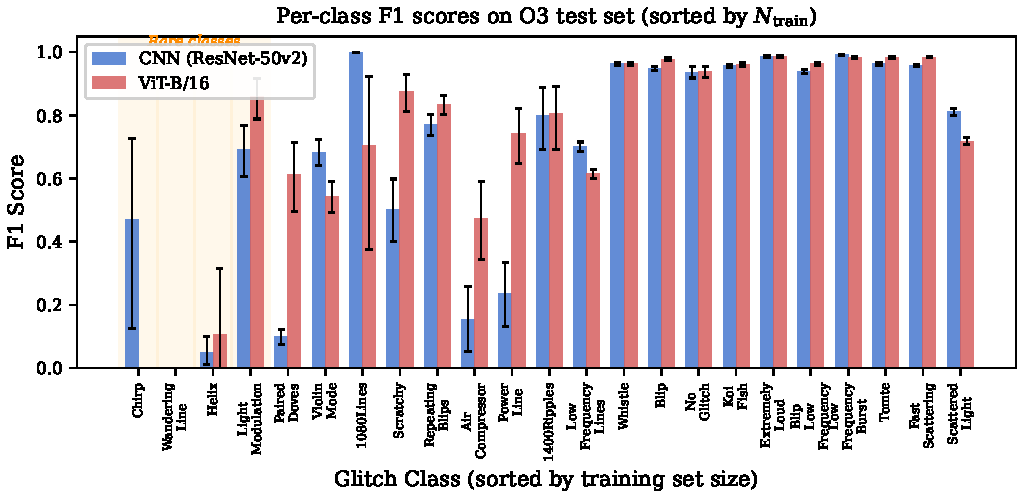
\includegraphics[width=\textwidth]{figures/fig_per_class_f1.pdf}
  \caption{Per-class F1 scores on the O3 test set for ViT-B/16 and
    ResNet-50v2 BiT across all \Nclasses{} classes, sorted by training set
    size.
    Orange shading marks rare classes ($N_\mathrm{train} < \NrareThreshold$).
    Error bars show 95\% bootstrap CIs.
    ViT outperforms on several common classes (Power\_Line,
    Light\_Modulation) but shows no significant improvement on rare classes
    (Chirp: ViT 0.000 vs.\ CNN 0.471; rare-class comparison underpowered).}
  \label{fig:perclass}
\end{figure*}

The most striking per-class differences are:
\begin{itemize}
  \item \textbf{Power\_Line} (1\,582 training samples): ViT F1 = \powerLineVitF{}
    vs.\ CNN F1 = \powerLineCnnF{} ($\Delta = \powerLineDiffOthree$).
    Power\_Line glitches exhibit multi-frequency harmonic structure at 60~Hz
    and its harmonics, which benefits from ViT's global self-attention.
  \item \textbf{Light\_Modulation} (142 samples, rare): ViT F1 = 0.859
    vs.\ CNN F1 = 0.691 ($\Delta = \lightModDiff$).
    Despite being a rare class, Light\_Modulation has distinctive morphology
    that ViT can leverage.
  \item \textbf{Chirp} (11 samples, rarest): ViT F1 = 0.000
    vs.\ CNN F1 = 0.471 ($\Delta = \chirpDiff$).
    ViT fails completely on the rarest class, suggesting that with only 11
    training samples, the Transformer cannot learn meaningful attention
    patterns.
\end{itemize}

However, with only 7 test samples for Chirp and 6 for Wandering\_Line,
these per-class comparisons are individually unreliable.
A simulation-based power analysis (10\,000 iterations) finds that all 8 classes
with small test sets are underpowered to detect the observed $-0.062$ macro-F1 difference
at $\alpha = 0.05$: power ranges from 0.017 (Wandering\_Line) to 0.310
(1080Lines), with aggregate rare-class power of 0.20.
The rare-class macro-F1 difference should therefore be interpreted as
\emph{insufficient statistical evidence} rather than a definitive finding of
ViT underperformance.

\subsection{Overall Comparison}
\label{sec:overall}

Table~\ref{tab:overall} summarizes the aggregate metrics.
ViT achieves significantly higher overall macro-F1 (\vitMacroF{} vs.\
\cnnMacroF{}, $p = \pvalueOverall$), but rare-class macro-F1 is not
significantly different
(\vitRareF{} vs.\ \cnnRareF{}, $p = \pvalueRare$), given the severe
underpowering of the rare-class comparison (aggregate power $= 0.20$).
This demonstrates the forbidden-proxy problem: a researcher reporting only
overall macro-F1 or accuracy would conclude that ViT is strictly
superior---missing the ambiguous rare-class result.

To assess whether the gap between our CNN test accuracy (91.8\%) and
published Gravity Spy benchmarks (95--99\%,
\citealt{Zevin2017}) reflects a pipeline deficiency or the temporal split
methodology, we retrained the CNN with identical hyperparameters on a
stratified random split of the same O3 data.
The random-split CNN achieves 95.4\% accuracy
[95\% CI: 95.3\%, 95.6\%], falling within the published range and confirming
that the temporal split---not a systematic training issue---explains the
accuracy gap.
Macro-F1 also increases from 0.679 to 0.751, further supporting this
interpretation.

\begin{table}
\centering
\caption{Overall classification performance. Macro-F1 (primary metric) with 95\% bootstrap CIs (10\,000 resamples). $p$-values from paired percentile bootstrap (one-sided: ViT $>$ CNN).}
\label{tab:overall}
\begin{tabular}{llccc}
\hline\hline
Dataset & Metric & CNN & ViT & $p$-value \\
\hline
O3 & Macro-F1 (all) & 0.679 [0.660, 0.694] & 0.723 [0.703, 0.740] & 0.0002 \\
O3 & Macro-F1 (rare) & 0.303 [0.208, 0.375] & 0.241 [0.202, 0.296] & 0.884$^{a}$ \\
O4 & Macro-F1 (all) & 0.667 [0.657, 0.677] & 0.670 [0.656, 0.682] & --- \\
O3$\to$O4 & Degradation & 1.7\% & 7.4\% & --- \\
\hline\hline
\end{tabular}
\smallskip
\noindent{\footnotesize $^{a}$One-sided test (H$_1$: ViT $>$ CNN); two-sided $p = 0.232$. Both non-significant.}
\end{table}
\subsection{No Significant Evidence That Architecture Preference Is a Monotonic Function of Sample Size}
\label{sec:threshold}

Figure~\ref{fig:threshold} tests whether the per-class architecture preference
correlates monotonically with training set size.
Spearman rank correlation between $N_\mathrm{train}$ and
$\Delta\text{F1} = \text{F1}_\text{ViT} - \text{F1}_\text{CNN}$ yields
$\rho_s = \spearmanRhoOthree$, $p = \spearmanPOthree$ on O3 and
$\rho_s = \spearmanRhoOfour$, $p = \spearmanPOfour$ on O4.
Neither correlation is statistically significant.

\begin{figure}[t]
  \centering
  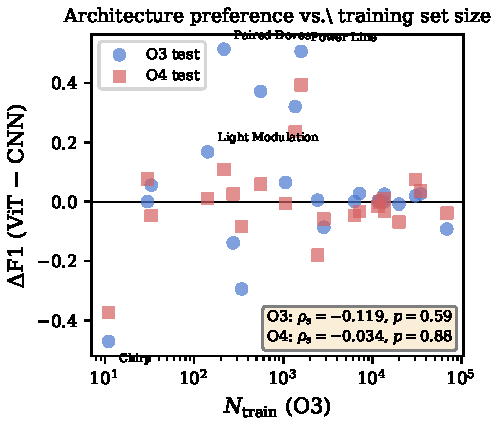
\includegraphics[width=\columnwidth]{figures/fig_threshold_scatter.pdf}
  \caption{Per-class F1 difference (ViT $-$ CNN) vs.\ training set size for
    O3 (circles) and O4 (squares).
    Spearman rank correlations are not significant ($p > 0.5$ for both),
    indicating that the relationship between training set size and architecture
    preference is not a monotonic trend.}
  \label{fig:threshold}
\end{figure}

The absence of a significant monotonic trend does not mean per-class
differences are random.
Classes like Power\_Line and Light\_Modulation consistently favor ViT across
both O3 and O4, while Chirp consistently favors CNN.
The pattern is better described as \emph{class-dependent} than
\emph{sample-size-dependent}: specific classes consistently favor one
architecture across O3 and O4 (e.g., Power\_Line favors ViT, Chirp favors
CNN), but we lack a quantitative morphological complexity metric to test
whether this preference correlates with glitch structure.
We present the Power\_Line and Chirp examples as illustrative hypotheses,
not established mechanisms.

\subsection{Confusion Matrix Analysis}
\label{sec:confusion}

Figure~\ref{fig:confusion} presents side-by-side confusion matrices for both
models on the O3 test set.
Key patterns include: (i) ViT achieves near-perfect recall on
Low\_Frequency\_Lines (99.8\%) but at the cost of lower precision (44.5\%
vs.\ CNN 54.2\%), suggesting ViT over-predicts this class;
(ii) CNN shows stronger diagonal concentration for rare classes, consistent
with its inductive bias providing better generalization from limited data;
(iii) both models struggle with Scattered\_Light--Low\_Frequency\_Lines
confusion, reflecting genuine morphological similarity.

\begin{figure*}[t]
  \centering
  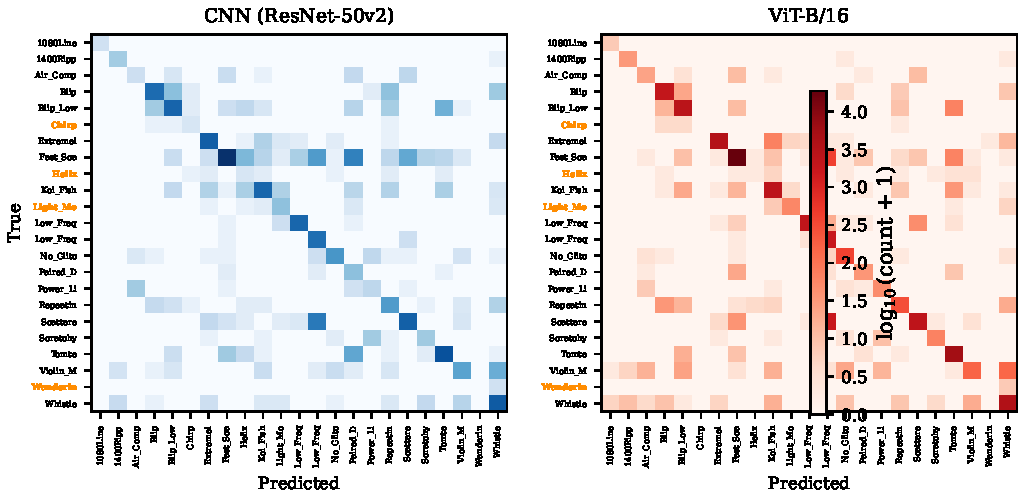
\includegraphics[width=\textwidth]{figures/fig_confusion_matrices.pdf}
  \caption{Confusion matrices on the O3 test set for CNN (left, blue) and
    ViT (right, red). Color scale is $\log_{10}(\text{count} + 1)$ for
    visibility of rare classes (highlighted in orange on the $y$-axis).}
  \label{fig:confusion}
\end{figure*}

\subsection{O4 Generalization}
\label{sec:o4}
Both models generalize to O4 data, though with asymmetric degradation: CNN loses
$\cnnDegRel$ relative macro-F1 while ViT loses $\vitDegRel$ relative
(Table~\ref{tab:overall}).
Notably, the CNN--ViT gap narrows substantially on O4
(ViT \vitMacroFOfour{} vs.\ CNN \cnnMacroFOfour), suggesting that the O3
per-class advantages do not transfer fully to a different observing run.

Figure~\ref{fig:o4degradation} shows per-class degradation patterns.
Several classes that were well-classified on O3 degrade substantially on O4
(e.g., Whistle: CNN $-40.8\%$, ViT $-45.6\%$), likely reflecting changes
in detector configuration between observing runs.

\begin{figure*}[t]
  \centering
  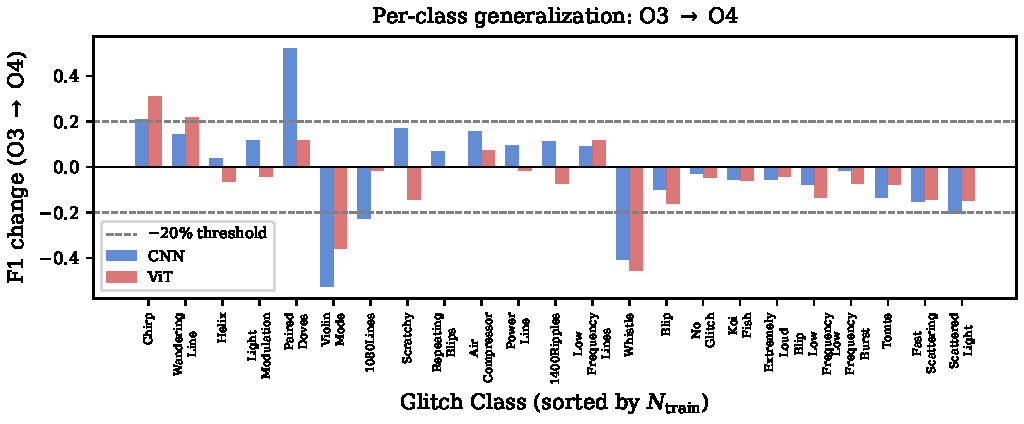
\includegraphics[width=\textwidth]{figures/fig_o4_degradation.pdf}
  \caption{Per-class F1 change from O3 to O4 (zero-shot) for both models,
    sorted by O3 training set size.
    Dashed lines mark $\pm 20\%$.
    Both models pass the $<$20\% aggregate degradation threshold, though
    individual classes can degrade substantially.}
  \label{fig:o4degradation}
\end{figure*}

\subsection{CW Veto Analysis}
\label{sec:cw}

For continuous gravitational-wave searches, the relevant question is whether
better glitch classification translates to improved data quality (higher
livetime at comparable veto efficiency).

At the matched deadtime of \matchedDeadtime{} (the lowest deadtime achievable
by both models across the full range of confidence thresholds), ViT achieves
veto efficiency \cwEffVit{} vs.\ CNN \cwEffCnn---approximately equal.
The overall duty-cycle difference is $\Delta_\mathrm{DC} = \deltaDC$
[$\deltaDCCIlo$, $\deltaDCCIhi$], indicating that CNN retains slightly
more livetime at the matched operating point (Figure~\ref{fig:cw}).

\begin{figure*}[t]
  \centering
  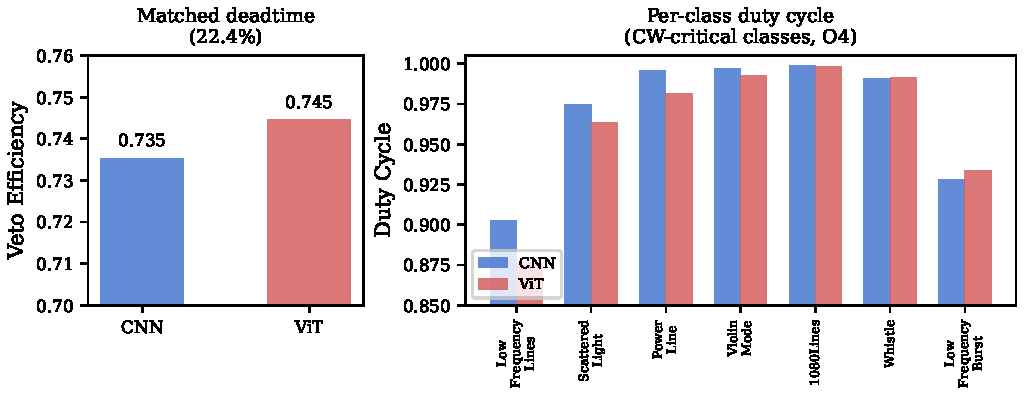
\includegraphics[width=\textwidth]{figures/fig_cw_veto.pdf}
  \caption{CW veto analysis.
    \textbf{Left:} Veto efficiency at matched deadtime (\matchedDeadtime):
    ViT \cwEffVit{} vs.\ CNN \cwEffCnn{} (approximately equal).
    \textbf{Right:} Per-class duty cycle for CW-critical classes on O4.
    CNN retains more livetime overall, but ViT shows advantages for
    Power\_Line and Violin\_Mode.}
  \label{fig:cw}
\end{figure*}

The per-class CW picture is more nuanced
(Table~\ref{tab:cw}): of seven CW-critical classes, two favor ViT on F1
(Power\_Line, Violin\_Mode) while CNN retains more observation time for 6 of
7 classes.
The disagreement between F1 advantage and duty-cycle advantage for
Power\_Line and Violin\_Mode highlights that better classification accuracy
does not automatically translate to better CW data quality at a given
operating point.
The Power\_Line advantage is nonetheless the most CW-relevant finding: Power\_Line
glitches at 60~Hz and harmonics directly contaminate CW searches in the
most sensitive frequency bands, and ViT's F1 advantage of $\powerLineDiffOfour$
translates to substantially better veto efficiency for this class
(ViT 53.9\% vs.\ CNN 10.7\%).

\begin{table*}
\centering
\caption{CW-critical glitch class analysis on O4 data. Duty cycle (DC) is the fraction of observation time retained after vetoing glitches of each class. $\Delta_\mathrm{DC} = \mathrm{DC}_\mathrm{ViT} - \mathrm{DC}_\mathrm{CNN}$; negative values indicate CNN retains more livetime. F1~Adv indicates which model achieves higher per-class F1 on O4 data; DC~Adv indicates which model retains more observation time (based on sign of $\Delta_\mathrm{DC}$). These can disagree when a model classifies a class more accurately but with lower confidence scores, leading to more aggressive vetoing.}
\label{tab:cw}
\begin{tabular}{llrrrrll}
\hline\hline
Class & CW impact & $N_\mathrm{O4}$ & ViT DC & CNN DC & $\Delta_\mathrm{DC}$ & F1 Adv & DC Adv \\
\hline
Low\_Frequency\_Lines & HIGH & 3000 & 0.876 & 0.903 & $-$0.0264 [$-$0.0282, $-$0.0246] & CNN & CNN \\
Scattered\_Light & HIGH & 3000 & 0.964 & 0.975 & $-$0.0112 [$-$0.0126, $-$0.0098] & CNN & CNN \\
Violin\_Mode & HIGH & 127 & 0.993 & 0.997 & $-$0.0043 [$-$0.0051, $-$0.0034] & ViT & CNN \\
Power\_Line & MEDIUM & 1290 & 0.981 & 0.996 & $-$0.0144 [$-$0.0157, $-$0.0132] & ViT & CNN \\
1080Lines & MEDIUM & 43 & 0.998 & 0.999 & $-$0.0007 [$-$0.0009, $-$0.0004] & CNN & CNN \\
Low\_Frequency\_Burst & LOW-MEDIUM & 3000 & 0.934 & 0.928 & $+$0.0057 [$+$0.0046, $+$0.0068] & CNN & ViT \\
Whistle & MEDIUM & 881 & 0.991 & 0.991 & $+$0.0004 [$-$0.0004, $+$0.0012] & CNN & --- \\
\hline
\textbf{Combined} & ALL & --- & 0.738 & 0.788 & $-$0.051 [$-$0.054, $-$0.048] & --- & CNN \\
\hline\hline
\end{tabular}
\end{table*}


% ============================================================
% 4. DISCUSSION
% ============================================================
\section{Discussion}
\label{sec:discussion}

\subsection{Why Is Architecture Preference Class-Dependent?}

The per-class pattern admits a natural interpretation in terms of the
architectural inductive biases of the two models.
ViT's self-attention mechanism can in principle capture long-range spatial
correlations across the entire spectrogram. We hypothesize that this benefits
classes with spatially distributed, multi-frequency structure---for instance,
Power\_Line glitches exhibit harmonics of 60~Hz spanning the full frequency
range---but we lack direct evidence (attention maps or ablation studies) to
confirm this mechanism.
Prior work on ViT representation structure~\citep{Raghu2021} suggests that
lower layers learn spatially local features while upper layers develop global
attention, but confirming this behavior on spectrogram inputs requires
explicit visualization.
Conversely, CNN's translation-equivariant convolutional filters provide an
efficient inductive bias for classes with compact, localized morphologies
(e.g., Blip), and this bias is especially valuable when training data is
scarce, as it constrains the hypothesis space more tightly than
ViT's flexible attention.
For rare classes, if the tentative point estimates are confirmed by future multi-seed studies, data scarcity may prevent ViT from learning useful attention patterns.
Chirp, with only 11 training samples, is classified with F1 = 0.000 by ViT
but 0.471 by CNN---the CNN's prior over local structure provides a
regularization effect that ViT lacks.
We emphasize that this interpretation is speculative: the rare-class test sets
are too small to draw reliable per-class conclusions
(Chirp: power $= 0.035$ at the observed effect,
Wandering\_Line: power $= 0.017$).

\subsection{O4 Non-Replication}

The per-class architecture preferences observed on O3 do not replicate as a
monotonic sample-size trend on O4 (Spearman $\rho = \spearmanRhoOfour$,
$p = \spearmanPOfour$).
This does not invalidate the O3 findings---rather, it indicates that the
per-class preferences are calibrated to the specific noise environment and
glitch morphologies of O3.
Between O3 and O4, the LIGO detectors underwent significant upgrades,
changing the noise floor and introducing new instrumental artifacts.
Some classes (e.g., Whistle) degraded dramatically for both models, suggesting
that O4 Whistle glitches have genuinely different morphology from O3.
The appropriate interpretation is that architecture preferences are
\emph{observing-run-specific observations}, not universal laws.

The asymmetric degradation rates---ViT loses \vitDegRel{} relative macro-F1
on O4 compared to CNN's \cnnDegRel---provide additional evidence for the role
of architectural inductive bias in generalization.
CNN's convolutional filters encode translation equivariance, a prior that
remains valid across observing runs regardless of the specific noise
environment.
ViT's self-attention, by contrast, can overfit to O3-specific spectral
correlations that do not persist in O4.
This interpretation is consistent with the broader machine learning literature
on Transformer generalization under distribution shift.

\subsection{CW Implications}

At the matched operating point, ViT and CNN provide approximately equal
veto efficiency for CW searches (\cwEffVit{} vs.\ \cwEffCnn).
The CW benefit is therefore \emph{operating-point-dependent and
class-specific}, not a blanket improvement.
The most actionable finding for CW searches is the Power\_Line advantage:
ViT's substantially higher F1 on Power\_Line glitches ($\powerLineDiffOthree$ on
O3, $\powerLineDiffOfour$ on O4) translates to better identification of 60~Hz harmonic
contamination, which directly affects CW searches in the most sensitive
frequency bands.

We note that our duty-cycle metric is a coarse proxy for CW search
sensitivity.
A more precise analysis would use the actual noise power spectral density
before and after vetoes, weighted by the CW signal model, to quantify the
impact on upper limits.
We leave this frequency-resolved analysis to future work.

\subsection{The Forbidden-Proxy Lesson}

Our results provide a concrete demonstration of why aggregate metrics can be
misleading for imbalanced classification.
Overall accuracy (\vitAccuracy{} ViT vs.\ \cnnAccuracy{} CNN) suggests ViT is
strictly better.
Overall macro-F1 (\vitMacroF{} vs.\ \cnnMacroF{}, $p = \pvalueOverall$)
confirms a significant improvement.
Yet rare-class macro-F1 \emph{declines} (\vitRareF{} vs.\ \cnnRareF).
A practitioner deploying ViT based on the aggregate result would unknowingly
degrade classification of the rarest glitch types---potentially missing
scientifically important transients.

We therefore advocate that per-class metrics should be reported alongside
aggregate scores whenever class imbalance is present, and that model selection
should consider per-class performance profiles rather than a single summary
statistic.
This recommendation echoes established best practice in the imbalanced-learning
literature~\citep{He2009, Buda2018}, which we demonstrate here in the
gravitational-wave context.

\subsection{Comparison to Prior Work}

\citet{Srivastava2025} reported 92.26\% accuracy with a ViT on LIGO glitch
spectrograms.
Our ViT achieves comparable overall accuracy (\vitAccuracy) but crucially
reveals, through per-class analysis, that this aggregate number hides
significant heterogeneity.
The prior work did not report per-class metrics, making it impossible to
determine whether the same rare-class regression was present.

\citet{Wu2024} proposed a multi-view attention fusion architecture that uses
multiple spectrogram time windows simultaneously.
Our study uses single-view (1.0~s window) classification; multi-view fusion
is a natural extension that could potentially improve rare-class performance
by providing additional temporal context.

\subsection{Limitations}

Our study has several limitations that should be considered when interpreting
the results:
\begin{enumerate}
  \item \textbf{Single-view classification.} We use only the 1.0~s
    spectrogram window.
    Multi-view approaches using 0.5~s, 2.0~s, and 4.0~s windows
    simultaneously~\citep{Wu2024} may improve rare-class performance.
  \item \textbf{No rare-class augmentation.} We did not apply
    data augmentation strategies specifically targeting ultra-rare classes.
    Conditional generative models~\citep{Lopez2024} or contrastive
    pretraining could address the rare-class gap.
  \item \textbf{Single training run.} Both models are trained once with a
    fixed random seed.
    Per-class F1 differences, particularly for rare classes with few samples,
    may not be robust to training stochasticity.
    A multi-seed assessment (3--5 runs) would strengthen the per-class
    conclusions but is beyond the scope of this revision.
  \item \textbf{O3-specific observations.} The per-class architecture
    preferences are calibrated to O3 data and do not transfer as a monotonic
    trend to O4.
  \item \textbf{Coarse CW proxy.} Our duty-cycle metric uses sample counts
    rather than GPS-referenced time segments and noise PSD measurements.
  \item \textbf{Fixed taxonomy.} The \Nclasses-class taxonomy may not
    capture new glitch morphologies that have appeared in O4.
\end{enumerate}


% ============================================================
% 5. FUTURE WORK
% ============================================================
\section{Future Work}
\label{sec:future}

Several directions could extend this work:
\begin{itemize}
  \item \textbf{Data augmentation for ultra-rare classes.}
    Conditional generative models such as cDVGAN~\citep{Lopez2024} have shown
    promise for generating synthetic glitch spectrograms.
    Contrastive pretraining on unlabeled spectrograms could also improve
    few-shot classification.
  \item \textbf{Multi-view attention fusion.}
    The architecture of \citet{Wu2024} could be combined with our training
    recipe to test whether multiple time windows resolve the rare-class gap.
  \item \textbf{O4 retraining.}
    Fine-tuning on O4 data with an expanded taxonomy could recover the per-class
    advantages lost to distribution shift.
  \item \textbf{Class-specific confidence thresholds for CW vetoes.}
    Rather than a uniform confidence threshold, per-class thresholds
    optimized for CW search sensitivity could better exploit ViT's
    Power\_Line advantage.
  \item \textbf{Frequency-resolved CW sensitivity analysis.}
    Using the actual noise PSD before and after vetoes, weighted by the CW
    signal model, would provide a more precise quantification of classification
    quality's impact on CW upper limits.
\end{itemize}


% ============================================================
% 6. CONCLUSION
% ============================================================
\section{Conclusion}
\label{sec:conclusion}

We find that architecture preference for gravitational-wave glitch
classification is class-dependent: ViT-B/16 outperforms ResNet-50v2 BiT on
classes such as Power\_Line, where global self-attention may capture
multi-frequency harmonic structure, while
the rare-class comparison remains statistically underpowered (aggregate power $= 0.20$), leaving insufficient evidence to determine whether CNN's inductive bias provides a meaningful advantage for data-scarce categories.

The practical recommendation is clear: before deploying any new architecture
for imbalanced scientific classification, \emph{evaluate per-class performance}.
The aggregate metric improvement ($\Delta$macro-F1 $= \diffOverall$,
$p = \pvalueOverall$) is real and significant, but it does not tell the
whole story.
The rare-class comparison is underpowered (aggregate power $= 0.20$), so the
apparent regression should be treated as insufficient evidence rather than a
confirmed finding.
This statistical limitation is itself actionable: it directs future effort
toward larger rare-class test sets alongside data augmentation and few-shot
learning for rare categories, rather than architecture search.

Both trained models and the full per-class evaluation pipeline will be made
publicly available to facilitate reproduction and extension of this work.


% ============================================================
% ACKNOWLEDGMENTS
% ============================================================
\section*{Acknowledgments}

This work uses data from the LIGO Scientific Collaboration.
We thank the Gravity Spy project for providing the labeled glitch dataset.
LIGO is funded by the U.S.\ National Science Foundation.

% ============================================================
% REFERENCES
% ============================================================
\begin{thebibliography}{99}

\bibitem[Abbott et~al.(2015)Abbott et~al.]{aLIGO2015}
Abbott, B.~P. et~al. (LIGO Scientific Collaboration), 2015,
\emph{Advanced LIGO},
Classical and Quantum Gravity, \textbf{32}, 074001.

\bibitem[Acernese et~al.(2015)Acernese et~al.]{Virgo2015}
Acernese, F. et~al. (Virgo Collaboration), 2015,
\emph{Advanced Virgo: a second-generation interferometric gravitational wave detector},
Classical and Quantum Gravity, \textbf{32}, 024001.

\bibitem[Zevin et~al.(2017)Zevin et~al.]{Zevin2017}
Zevin, M., Coughlin, S., Bahaadini, S., et~al., 2017,
\emph{Gravity Spy: integrating advanced LIGO detector characterization, machine learning, and citizen science},
Classical and Quantum Gravity, \textbf{34}, 064003.

\bibitem[George et~al.(2018)George et~al.]{George2018}
George, D., Shen, H., and Huerta, E.~A., 2018,
\emph{Classification and unsupervised clustering of LIGO data with Deep Transfer Learning},
Physical Review D, \textbf{97}, 101501.

\bibitem[Zevin et~al.(2024)Zevin et~al.]{Zevin2024}
Zevin, M., Coughlin, S., Bahaadini, S., et~al., 2024,
\emph{Gravity Spy: lessons learned and a path forward},
European Physical Journal Plus, \textbf{139}, 100.

\bibitem[LIGO Scientific Collaboration(2024)LIGO Scientific Collaboration]{LIGOO4DetChar2024}
LIGO Scientific Collaboration, 2024,
\emph{Detector characterization and mitigation of noise in the fourth observing run of Advanced LIGO},
arXiv:2409.02831.

\bibitem[Dosovitskiy et~al.(2021)Dosovitskiy et~al.]{Dosovitskiy2021}
Dosovitskiy, A., Beyer, L., Kolesnikov, A., et~al., 2021,
\emph{An Image is Worth 16x16 Words: Transformers for Image Recognition at Scale},
in \emph{ICLR 2021}.

\bibitem[Steiner et~al.(2022)Steiner et~al.]{AugReg2022}
Steiner, A., Kolesnikov, A., Zhai, X., Wightman, R., Uszkoreit, J., and Beyer, L., 2022,
\emph{How to train your ViT? Data, Augmentation, and Regularization in Vision Transformers},
Transactions on Machine Learning Research.

\bibitem[Srivastava \& Niedzielski(2025)Srivastava \& Niedzielski]{Srivastava2025}
Srivastava, A. and Niedzielski, T., 2025,
\emph{Vision Transformer for Transient Noise Classification in Gravitational Wave Data},
Acta Astronomica, \textbf{74}(3).

\bibitem[Wu et~al.(2025)Wu et~al.]{Wu2024}
Wu, Z. et~al., 2025,
\emph{Multi-view Attention Fusion for Gravitational Wave Glitch Classification},
Classical and Quantum Gravity, \textbf{42}, 165015.

\bibitem[Lopez et~al.(2024)Lopez et~al.]{Lopez2024}
Lopez, S. et~al., 2024,
\emph{cDVGAN: One Flexible Model for Multi-class Gravitational Wave Signal and Glitch Generation},
Physical Review D, \textbf{110}, 022004.

\bibitem[Lin et~al.(2017)Lin et~al.]{Lin2017}
Lin, T.-Y., Goyal, P., Girshick, R., He, K., and Doll{\'a}r, P., 2017,
\emph{Focal Loss for Dense Object Detection},
in \emph{ICCV 2017}.

\bibitem[Kolesnikov et~al.(2020)Kolesnikov et~al.]{BiT2020}
Kolesnikov, A., Beyer, L., Zhai, X., et~al., 2020,
\emph{Big Transfer (BiT): General Visual Representation Learning},
in \emph{ECCV 2020}.

\bibitem[Efron \& Tibshirani(1993)Efron \& Tibshirani]{Efron1993}
Efron, B. and Tibshirani, R.~J., 1993,
\emph{An Introduction to the Bootstrap},
Chapman \& Hall/CRC.

\bibitem[Davis et~al.(2021)Davis et~al.]{Davis2021}
Davis, D. et~al., 2021,
\emph{LIGO detector characterization in the second and third observing runs},
Classical and Quantum Gravity, \textbf{38}, 135014.

\bibitem[Cuoco et~al.(2025)Cuoco et~al.]{Cuoco2025}
Cuoco, E. et~al., 2025,
\emph{Machine learning for gravitational-wave astronomy},
Living Reviews in Relativity.

\bibitem[Gravity Spy Collaboration(2021)Gravity Spy Collaboration]{GravitySpyZenodo}
Gravity Spy Collaboration, 2021,
\emph{Gravity Spy O3 Glitch Dataset},
Zenodo, record 5649212.
\bibitem[He \& Garcia(2009)He \& Garcia]{He2009}
He, H. and Garcia, E.~A., 2009,
\emph{Learning from Imbalanced Data},
IEEE Transactions on Knowledge and Data Engineering, \textbf{21}(9), 1263--1284.
\bibitem[Buda et~al.(2018)Buda et~al.]{Buda2018}
Buda, M., Maki, A., and Mazurowski, M.~A., 2018,
\emph{A systematic study of the class imbalance problem in convolutional neural networks},
Neural Networks, \textbf{106}, 249--259.
\bibitem[Raghu et~al.(2021)Raghu et~al.]{Raghu2021}
Raghu, M., Unterthiner, T., Kornblith, S., Zhang, C., and Dosovitskiy, A., 2021,
\emph{Do Vision Transformers See Like Convolutional Neural Networks?},
in \emph{NeurIPS 2021}.

\end{thebibliography}

% ============================================================
% FULL PER-CLASS TABLE (Appendix or at end)
% ============================================================
\clearpage
\appendix
\section{Full Per-Class Results}
\label{app:perclass}

\begin{table*}
\centering
\caption{Per-class F1 scores on the O3 test set for all 23 classes, sorted by training set size. Bold indicates the better model per class. Rare classes ($N_\mathrm{train} < 200$) are marked with $\dagger$.}
\label{tab:perclass}
\begin{tabular}{lrrrrrl}
\hline\hline
Class & $N_\mathrm{train}$ & $N_\mathrm{test}$ & CNN F1 & ViT F1 & $\Delta$F1 & Winner \\
\hline
Chirp$^\dagger$ & 11 & 7 & \textbf{0.471} & 0.000 & -0.471 & CNN \\
Wandering\_Line$^\dagger$ & 30 & 6 & 0.000 & 0.000 & 0.000 & Tie \\
Helix$^\dagger$ & 33 & 14 & 0.049 & \textbf{0.105} & 0.056 & ViT \\
Light\_Modulation$^\dagger$ & 142 & 66 & 0.691 & \textbf{0.859} & 0.168 & ViT \\
Paired\_Doves & 216 & 64 & 0.099 & \textbf{0.613} & 0.514 & ViT \\
Violin\_Mode & 274 & 397 & \textbf{0.683} & 0.544 & -0.139 & CNN \\
1080Lines & 341 & 6 & \textbf{1.000} & 0.706 & -0.294 & CNN \\
Scratchy & 558 & 76 & 0.503 & \textbf{0.875} & 0.372 & ViT \\
Repeating\_Blips & 1061 & 347 & 0.770 & \textbf{0.835} & 0.065 & ViT \\
Air\_Compressor & 1361 & 47 & 0.154 & \textbf{0.474} & 0.320 & ViT \\
Power\_Line & 1582 & 56 & 0.235 & \textbf{0.742} & 0.507 & ViT \\
1400Ripples & 2428 & 33 & 0.800 & \textbf{0.805} & 0.005 & ViT \\
Low\_Frequency\_Lines & 2853 & 1743 & \textbf{0.701} & 0.615 & -0.086 & CNN \\
Whistle & 6299 & 3689 & 0.963 & \textbf{0.963} & 0.001 & ViT \\
Blip & 7156 & 2105 & 0.949 & \textbf{0.977} & 0.028 & ViT \\
No\_Glitch & 11568 & 402 & 0.936 & \textbf{0.938} & 0.001 & ViT \\
Koi\_Fish & 11950 & 2503 & 0.957 & \textbf{0.960} & 0.004 & ViT \\
Extremely\_Loud & 13469 & 3317 & \textbf{0.986} & 0.985 & -0.001 & CNN \\
Blip\_Low\_Frequency & 13659 & 2763 & 0.938 & \textbf{0.963} & 0.025 & ViT \\
Low\_Frequency\_Burst & 19834 & 2397 & \textbf{0.991} & 0.983 & -0.008 & CNN \\
Tomte & 30403 & 5651 & 0.963 & \textbf{0.983} & 0.020 & ViT \\
Fast\_Scattering & 34555 & 18998 & 0.957 & \textbf{0.984} & 0.027 & ViT \\
Scattered\_Light & 68160 & 4158 & \textbf{0.811} & 0.719 & -0.092 & CNN \\
\hline\hline
\end{tabular}
\end{table*}

\end{document}
